\documentclass{article}
\usepackage[utf8]{inputenc}
\usepackage{a4wide}


%% Copy the following definitions into your preamble. Then copy the
%% tikz figures into your main document and replace "xxx" in the calls
%% to \statelabel and \edgelabel with the correct costs.


\usepackage{tikz}
\usetikzlibrary{matrix,calc,positioning,patterns}
\usetikzlibrary{arrows,automata}

\tikzstyle{annotated states}=[
    ->,>=stealth',auto,node distance=3em and 0.5em,
    every node/.style={
        align=center,
    },
    every state/.style={
        circle split,
        minimum size=12mm,
}]
\newcommand{\statelabel}[2]{\ensuremath{#1}\nodepart{lower}\ensuremath{#2}}
\newcommand{\edgelabel}[2]{\ensuremath{#1}\\\ensuremath{#2}}


\begin{document}
    \begin{center}
    \small
    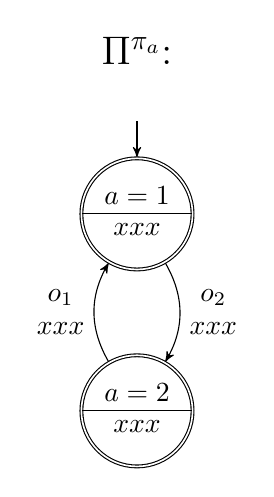
\begin{tikzpicture}[annotated states, baseline]
        \node (label) {\Large $\Pi^{\pi_a}$:};
        \node[initial above, initial text=, state, accepting, below=of label] (s1) {\statelabel{a=1}{xxx}};
        \node[state, accepting, below=of s1] (s2) {\statelabel{a=2}{xxx}};

        \path
            (s2) edge[bend left] node {\edgelabel{o_1}{xxx}} (s1)
            (s1) edge[bend left] node {\edgelabel{o_2}{xxx}} (s2)
        ;
    \end{tikzpicture}
    \qquad
    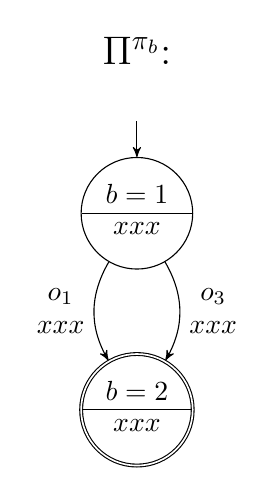
\begin{tikzpicture}[annotated states, baseline]
        \node (label) {\Large $\Pi^{\pi_b}$:};
        \node[initial above, initial text=, state, below=of label] (s1) {\statelabel{b=1}{xxx}};
        \node[state, accepting, below=of s1] (s2) {\statelabel{b=2}{xxx}};

        \path
            (s1) edge[bend right] node[swap] {\edgelabel{o_1}{xxx}} (s2)
            (s1) edge[bend left] node {\edgelabel{o_3}{xxx}} (s2)
        ;
    \end{tikzpicture}
    \qquad
    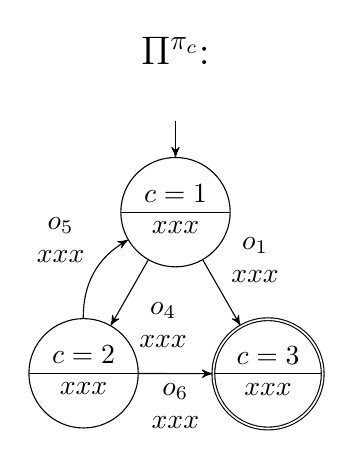
\begin{tikzpicture}[annotated states, baseline]
        \node (label) {\Large $\Pi^{\pi_c}$:};
        \node[initial above, initial text=, state, below=of label] (s1) {\statelabel{c=1}{xxx}};
        \node[state, below left=of s1] (s2) {\statelabel{c=2}{xxx}};
        \node[state, accepting, below right=of s1] (s3) {\statelabel{c=3}{xxx}};

        \path
            (s1) edge node {\edgelabel{o_1}{xxx}} (s3)
            (s1) edge node {\edgelabel{o_4}{xxx}} (s2)
            (s2) edge[bend left] node {\edgelabel{o_5}{xxx}} (s1)
            (s2) edge node[swap] {\edgelabel{o_6}{xxx}} (s3)
        ;
    \end{tikzpicture}
    \qquad
    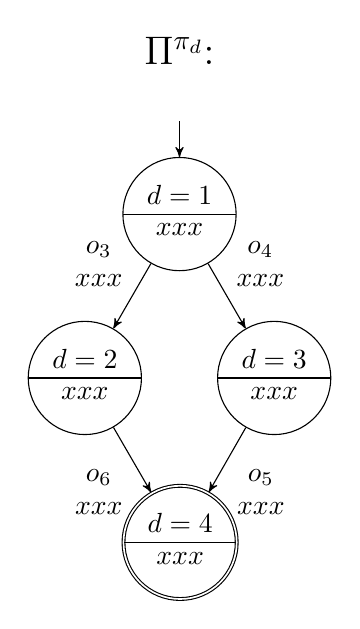
\begin{tikzpicture}[annotated states, baseline]
        \node (label) {\Large $\Pi^{\pi_d}$:};
        \node[initial above, initial text=, state, below=of label] (s1) {\statelabel{d=1}{xxx}};
        \node[state, below left=of s1] (s2) {\statelabel{d=2}{xxx}};
        \node[state, below right=of s1] (s3) {\statelabel{d=3}{xxx}};
        \node[state, accepting, below right=of s2] (s4) {\statelabel{d=4}{xxx}};

        \path
            (s1) edge node[swap] {\edgelabel{o_3}{xxx}} (s2)
            (s1) edge node {\edgelabel{o_4}{xxx}} (s3)
            (s3) edge node {\edgelabel{o_5}{xxx}} (s4)
            (s2) edge node[swap] {\edgelabel{o_6}{xxx}} (s4)
        ;
    \end{tikzpicture}
    \end{center}
\end{document}
